\documentclass[10pt,twocolumn,a4paper]{article}

\usepackage[utf8]{inputenc}
\usepackage[T1]{fontenc}
\usepackage[a4paper,margin=1in]{geometry}
\usepackage{parskip}
\usepackage{titlesec}
\usepackage{xcolor}
\usepackage{listings}
\usepackage{cite}
\usepackage{url}
\usepackage{tikz}
\usetikzlibrary{positioning,calc,arrows}
\usepackage[hidelinks]{hyperref}

% --- shared diagram styles ---------------------------------------------------
\newcommand{\dstyles}{%
  \tikzset{%
    pstep/.style={draw, rounded corners, fill=black!4, align=left,
      inner sep=5pt, font=\footnotesize, text width=6.2cm},
    flow/.style={->, >=latex, thick},
    memblock/.style={draw, align=left, inner sep=5pt,
      font=\footnotesize\ttfamily, fill=black!3},
  }%
}

% --- listing style for the few assembly / code fragments that are genuinely
%     part of the argument, not documentation ---------------------------------
\definecolor{codegray}{gray}{0.95}
\lstset{
  basicstyle=\ttfamily\small,
  backgroundcolor=\color{codegray},
  frame=single,
  framesep=4pt,
  xleftmargin=4pt,
  breaklines=true,
  columns=fullflexible,
  keepspaces=true,
}

\titleformat{\section}{\normalfont\Large\bfseries}{\thesection}{0.6em}{}
\titleformat{\subsection}{\normalfont\large\bfseries}{\thesubsection}{0.6em}{}

\title{\textbf{Design and Implementation of a Linux Process\\
Manipulation and Runtime Analysis Tool}}
\author{}
\date{}

\begin{document}

% ---------------------------------------------------------------------------
% Title page
% ---------------------------------------------------------------------------
\begin{titlepage}
  \centering
  \vspace*{1cm}
  {\large TOROS UNIVERSITY\par}
  {\large ENGINEERING FACULTY\par}
  {\large DEPARTMENT OF SOFTWARE ENGINEERING\par}
  \vspace{2cm}
  {\large SWE403 --- GRADUATION THESIS\par}
  \vspace{2cm}
  {\LARGE\bfseries Design and Implementation of a Linux Process
    Manipulation and Runtime Analysis Tool\par}
  \vspace{2.5cm}
  {\large By\par}
  \vspace{0.3cm}
  {\large 21506008\par}
  {\large Ula\c{s} Tan Ersoyak\par}
  \vfill
  {\large 2025\par}
\end{titlepage}

% ---------------------------------------------------------------------------
% Abstract
% ---------------------------------------------------------------------------
\onecolumn
\begin{abstract}
\noindent
This thesis investigates how a running program on Linux can be inspected and
modified from the outside, and it does so by building a tool---\emph{Process
Processor} (\texttt{pp})---from first principles rather than by using an
existing debugger. The central research question is whether the three
capabilities usually provided by separate, mature tools---memory inspection,
runtime code modification, and symbol-level analysis---can be reconstructed on
top of only the primitive interfaces the kernel exposes (\texttt{ptrace}, the
\texttt{/proc} filesystem, the cross-process memory system calls, and the ELF
format), and what the attempt reveals about the boundary the operating system
enforces between processes. A recurring mechanism underlies every modification
feature: because a process may only allocate or re-protect its \emph{own}
address space, \texttt{pp} makes the target execute the required system call on
its own behalf by hijacking a thread's registers, planting a small instruction
stub, and regaining control through a breakpoint. The tool implements this
mechanism for memory allocation (\texttt{mmap}), permission changes
(\texttt{mprotect}), shared-library injection (\texttt{dlopen}), and function
hooking. The evaluation shows that the inspection and injection features are
reliable, while function hooking succeeds only for self-contained functions:
the experiment exposes relocation and stack-alignment problems that are
intrinsic to code injection rather than incidental to the implementation. The
work is therefore presented as a study of the mechanisms and their limits, not
as a production debugger.
\end{abstract}

\vspace{0.5cm}
\noindent\textbf{Keywords:} Linux, process manipulation, runtime analysis,
\texttt{ptrace}, \texttt{/proc}, ELF, memory management, code injection,
function hooking, disassembly.

\vspace{1em}
\tableofcontents
\twocolumn

% ===========================================================================
\section{Introduction}
% ===========================================================================

\subsection{Motivation}
Understanding how a program behaves while it is running is a recurring need in
debugging, security analysis, and systems education. The state that matters at
run time---the contents of memory, the layout of code, the register context of
each thread---is not visible in the source and only partially visible in the
binary. Linux exposes this state, and the means to change it, through a small
set of low-level interfaces: the \texttt{/proc} filesystem, the \texttt{ptrace}
system call, the cross-process memory calls \texttt{process\_vm\_readv} and
\texttt{process\_vm\_writev}, and the ELF format that describes every
executable and shared object. Mature tools such as debuggers and dynamic
instrumentation frameworks are built on exactly these interfaces, but they
present them behind large abstractions that hide the underlying mechanics. The
mechanics themselves---how one process is allowed to read another's memory, why
it cannot simply change that memory's permissions, how a function can be
redirected while the program runs---are what this thesis sets out to examine.

\subsection{Problem Statement}
A debugger or an instrumentation framework answers the question ``what is this
program doing?'' but does not, by its nature, explain \emph{how} the answer is
obtained. The operating system deliberately isolates processes from one
another; any tool that inspects or alters a foreign process must work within,
and occasionally around, that isolation. The problem addressed here is to make
those boundary-crossing mechanisms explicit by implementing them directly,
and to establish where they hold and where they break down. Rather than
consume an existing abstraction, this work reconstructs one, so that each
capability corresponds to a concrete, inspectable use of a kernel interface.

\subsection{Research Questions}
The thesis is organised around three questions:
\begin{enumerate}
  \item \textbf{RQ1.} Can memory inspection, symbol-level program analysis, and
  runtime code modification be built on the primitive Linux interfaces alone,
  without relying on an existing debugger?
  \item \textbf{RQ2.} Given that a process may modify only its own address
  space, by what mechanism can an external tool cause a target to allocate
  memory, change permissions, and load code on its own behalf---and is that
  mechanism uniform across these operations?
  \item \textbf{RQ3.} Where are the practical limits of external code
  modification, and are those limits a property of the implementation or of the
  technique itself?
\end{enumerate}

\subsection{Contributions}
The thesis makes the following contributions:
\begin{itemize}
  \item A single tool, \texttt{pp}, that unifies memory inspection,
  symbol resolution, disassembly, and runtime code modification over a common
  model of processes and memory regions, implemented directly on kernel
  interfaces.
  \item An account of a \emph{uniform injection mechanism}---register hijack,
  instruction-stub insertion, and breakpoint return---shown to serve
  \texttt{mmap}, \texttt{mprotect}, and \texttt{dlopen} alike.
  \item A qualitative evaluation that separates the capabilities which work
  reliably from function hooking, which does not, and attributes the difference
  to relocation and stack alignment rather than to defects in the code.
\end{itemize}

\subsection{Organisation}
Section~\ref{sec:background} reviews the interfaces the tool depends on and
positions \texttt{pp} against existing tools. Section~\ref{sec:design}
describes the design and the methodology, centred on the injection mechanism.
Section~\ref{sec:impl} details the implementation of the inspection and
modification features. Section~\ref{sec:eval} evaluates the result and
discusses the limits that emerged. Section~\ref{sec:conclusion} returns to the
research questions.

% ===========================================================================
\section{Background and Related Work}\label{sec:background}
% ===========================================================================

\subsection{Interfaces for External Process Access}
Only the facts that the rest of the thesis relies on are summarised here; the
manual pages are the authoritative reference.

\textbf{The \texttt{/proc} filesystem} presents kernel state as files. Each
process has a directory \texttt{/proc/[pid]}; \texttt{pp} reads \texttt{comm}
for the process name, \texttt{maps} for the list of mapped memory regions (each
with an address range, permission bits \texttt{rwxp}, and an optional backing
file), \texttt{statm} for resident-memory accounting, \texttt{exe} for the
executable path, and the \texttt{task/} subdirectory to enumerate
threads.

\textbf{Cross-process memory access.} \texttt{process\_vm\_readv} and
\texttt{process\_vm\_writev} copy data directly between the address spaces of
two processes without trapping through \texttt{/proc/[pid]/mem}, subject to the
same permission checks. \texttt{pp} uses them for all bulk reads
and writes of target memory.

\textbf{Process control.} \texttt{ptrace} lets a tracer attach to a thread,
stop it, read and write its registers (\texttt{PTRACE\_GETREGS} /
\texttt{PTRACE\_SETREGS}), read and write individual words of its memory
(\texttt{PTRACE\_PEEKTEXT} / \texttt{PTRACE\_POKETEXT}), and resume
it. This register- and word-level control is what makes the
injection mechanism of Section~\ref{sec:design} possible.

\textbf{The isolation boundary.} A process may allocate memory
(\texttt{mmap}) or change the protection of a region
(\texttt{mprotect}) only within its own address space; there is
no system call that lets one process do this to another. This single
restriction is the reason the tool cannot simply ``allocate memory in the
target'' and instead must make the target perform the call itself---the pivot
on which the design turns.

\textbf{ELF.} Executables and shared objects carry symbol tables
(\texttt{.symtab}/\texttt{.dynsym} with their string tables) that map function
names to addresses, and program headers whose first \texttt{PT\_LOAD} segment
fixes the load bias needed to translate a symbol's value into a runtime
address. \texttt{pp} parses these structures directly to resolve
functions.

\subsection{Existing Tools and Positioning}
Several categories of tool already perform parts of what \texttt{pp} does.
General-purpose debuggers such as GDB are built on \texttt{ptrace} and provide
breakpoints, memory inspection, and symbol resolution, but as general systems
they hide these mechanisms behind a command language and a large runtime.
Tracers such as \texttt{strace} and \texttt{ltrace} observe system and library
calls without modifying behaviour. The loader-level technique of
\texttt{LD\_PRELOAD} interposes replacement functions, but only at process
start and only for dynamically resolved symbols. Dynamic instrumentation
frameworks, ranging from academic systems such as Pin~\cite{pin}, which rewrites
a program's instruction stream through a just-in-time compiler, to production
tools such as Frida, inject substantial machinery into the target and expose a
high-level API for hooking and tracing. Memory scanners and ``trainers''
such as \texttt{scanmem} and Cheat Engine specialise in searching and editing
live memory values but do not perform code injection or symbol analysis.

\texttt{pp} is not intended to compete with any of these. Its distinguishing
choice is pedagogical: it reconstructs inspection, analysis, and modification
\emph{from the primitives}, in one small codebase, so that each feature is a
visible use of a kernel interface rather than a call into an abstraction. The
uniform injection mechanism that this exercise surfaces (Section~\ref{sec:design})
is the technical core; the breadth of commands is secondary.

% ===========================================================================
\section{Design and Methodology}\label{sec:design}
% ===========================================================================

\subsection{Design Goals}
The tool was built to satisfy three goals derived from the research questions:
every feature should rest on a primitive interface rather than on another tool;
the modification features should share one mechanism rather than each inventing
its own; and the model of a process and its memory should be uniform enough that
inspection, analysis, and modification operate on the same abstractions. The
development method was iterative and exploratory---each feature was implemented
against a live process and validated by observation---which is appropriate for a
study whose aim is to understand mechanisms and expose their limits rather than
to meet a fixed specification.

\subsection{Architecture}
\texttt{pp} is organised into a small number of modules with clear
responsibilities. A \texttt{process} abstraction represents a target and owns
everything derivable from \texttt{/proc} and the on-disk binary: its name,
memory regions, threads, base address, and resolved functions. A
\texttt{memory\_region} abstraction models one mapped range---its bounds,
permissions, and backing name---and is the common currency of every memory
operation. A \texttt{debugger} abstraction holds an active \texttt{ptrace}
attachment to every thread of the target and implements the operations that
require control of execution: reading and writing registers, allocating memory,
changing permissions, injecting a library, and hooking a function. Supporting
modules provide disassembly (a thin wrapper over the Capstone
framework), the command-line interface, and utilities for ELF
and file handling. The separation lets the same region and process model serve a
read-only inspection command and a destructive modification command without
special-casing.

\subsection{The Uniform Injection Mechanism}\label{sec:mechanism}
The isolation boundary described in Section~\ref{sec:background} means that
operations like ``allocate a page in the target'' or ``make this region
executable'' cannot be issued from the tool. The design answer, and the single
most important idea in the implementation, is to make the \emph{target} issue
the call while the tool choreographs it. The procedure, shown in
Figure~\ref{fig:inject}, is identical for every such operation:

\begin{enumerate}
  \item Attach to and stop the target's main thread; save its registers.
  \item Locate an executable region and save the machine-code word at its start.
  \item Overwrite that word with a short stub: the instruction that performs the
  operation, followed by an \texttt{int3} breakpoint (\texttt{0xCC}) and
  \texttt{nop} padding.
  \item Set the registers so that the instruction pointer points at the stub and
  the argument registers follow the relevant calling convention.
  \item Resume the thread and \texttt{waitpid} for it to hit the breakpoint.
  \item Read the result from the register file, then restore both the saved
  registers and the saved code word, leaving the target as it was found.
\end{enumerate}

\begin{figure}[t]
\centering
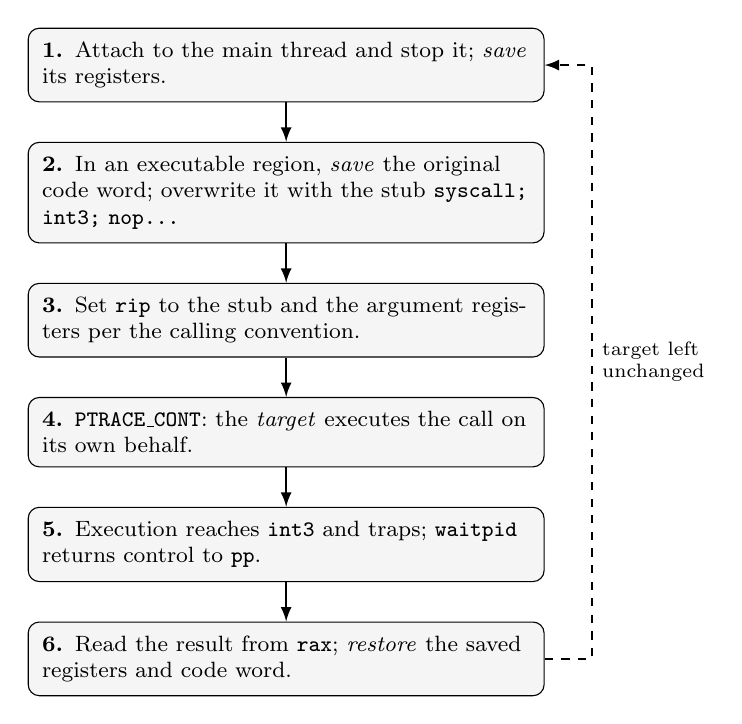
\begin{tikzpicture}[node distance=5mm]
  \dstyles
  \node[pstep] (s1) {\textbf{1.} Attach to the main thread and stop it;
    \emph{save} its registers.};
  \node[pstep, below=of s1] (s2) {\textbf{2.} In an executable region, \emph{save}
    the original code word; overwrite it with the stub
    \texttt{syscall; int3; nop\dots}};
  \node[pstep, below=of s2] (s3) {\textbf{3.} Set \texttt{rip} to the stub and the
    argument registers per the calling convention.};
  \node[pstep, below=of s3] (s4) {\textbf{4.} \texttt{PTRACE\_CONT}: the
    \emph{target} executes the call on its own behalf.};
  \node[pstep, below=of s4] (s5) {\textbf{5.} Execution reaches \texttt{int3} and
    traps; \texttt{waitpid} returns control to \texttt{pp}.};
  \node[pstep, below=of s5] (s6) {\textbf{6.} Read the result from \texttt{rax};
    \emph{restore} the saved registers and code word.};
  \draw[flow] (s1) -- (s2);
  \draw[flow] (s2) -- (s3);
  \draw[flow] (s3) -- (s4);
  \draw[flow] (s4) -- (s5);
  \draw[flow] (s5) -- (s6);
  \draw[flow, dashed] (s6.east) -- ++(6mm,0) |- node[pos=0.25,right,font=\scriptsize,align=left]
    {target left\\ unchanged} (s1.east);
\end{tikzpicture}
\caption{The uniform injection mechanism. Steps 1--3 and~6 are performed by
\texttt{pp} through \texttt{ptrace}; steps 4--5 run inside the target. The same
cycle serves \texttt{mmap}, \texttt{mprotect}, and \texttt{dlopen}, differing
only in the stub and the register setup.}
\label{fig:inject}
\end{figure}

For a system call the stub is simply \texttt{syscall; int3}, assembled as the
word \texttt{0x90909090CC050F} (\texttt{0F 05} followed by \texttt{CC} and
padding), with \texttt{rax} set to the syscall number and \texttt{rdi},
\texttt{rsi}, \texttt{rdx}, \texttt{r10}, \texttt{r8}, \texttt{r9} set to its
arguments. Allocation sets \texttt{rax} to the \texttt{mmap} number and lets the
kernel choose an address; a permission change sets it to the \texttt{mprotect}
number with the target region's bounds and the desired protection. The breakpoint
is what returns control: it stops the target and hands the tool a defined point at
which to read the return value and undo the modification. Because the mechanism
is uniform, adding a new privileged operation is a matter of choosing the stub and
the register setup rather than designing a new technique.

\subsection{Modification Strategies Built on the Mechanism}
Two higher-level features extend the mechanism beyond a single system call.

\emph{Shared-library injection} causes the target to call \texttt{dlopen} on a
path the tool has written into target memory. Here the stub is a \texttt{call}
through a register holding the resolved \texttt{dlopen} address rather than a
\texttt{syscall}, and a freshly allocated region is used as a clean stack so that
the call has somewhere to push its return address. Using the target's own
dynamic linker means the injected library is loaded exactly as if it had been
present at start-up, including the execution of its constructors, and can be
unloaded again---making this the least invasive modification strategy.

\emph{Function hooking} redirects a function to replacement code. The replacement
is written as an ordinary C++ source file exposing a \texttt{hook\_main} symbol;
\texttt{pp} compiles it, extracts just that function's bytes from the resulting
ELF, allocates an executable page in the target, writes the code there, and
finally overwrites the prologue of the target function with a sequence that loads
the replacement's address and jumps to it (Figure~\ref{fig:hook}). This is the
classic in-place interception approach popularised by Detours~\cite{detours}; it
is the most invasive strategy and, as Section~\ref{sec:eval} shows, the one whose
assumptions are most easily violated.

\begin{figure}[t]
\centering
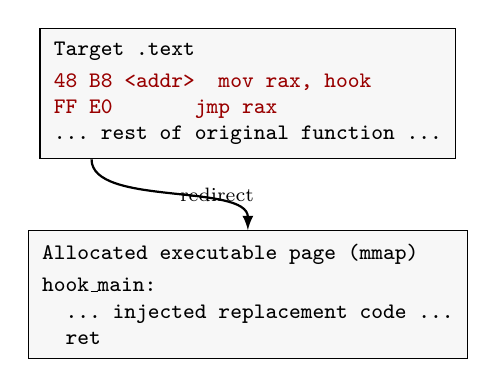
\begin{tikzpicture}[node distance=9mm]
  \dstyles
  \node[memblock, align=left] (t) {%
    \textbf{Target \texttt{.text}}\\[2pt]
    \textcolor{red!60!black}{48 B8 <addr>\ \ mov rax, hook}\\
    \textcolor{red!60!black}{FF E0\ \ \ \ \ \ \ jmp rax}\\
    \ldots\ rest of original function \ldots};
  \node[memblock, below=of t] (h) {%
    \textbf{Allocated executable page (mmap)}\\[2pt]
    hook\_main:\\
    \ \ \ldots\ injected replacement code \ldots\\
    \ \ ret};
  \draw[flow] ($(t.south west)!0.25!(t.south)$) .. controls +(0,-6mm) and +(0,6mm)
    .. node[right,font=\scriptsize]{redirect} (h.north);
\end{tikzpicture}
\caption{Function hooking. The first bytes of the target function are overwritten
with \texttt{mov rax, <hook>; jmp rax}, redirecting execution into a page holding
the extracted \texttt{hook\_main} code. The overwritten prologue bytes are not
relocated elsewhere, which is the source of the limitations in
Section~\ref{sec:eval}.}
\label{fig:hook}
\end{figure}

% ===========================================================================
\section{Implementation}\label{sec:impl}
% ===========================================================================
This section records the implementation decisions that are not obvious from the
mechanism itself. It deliberately omits the catalogue of command-line commands,
which is operational detail rather than a research result.

\subsection{Memory Inspection}
Reads and writes of target memory go through \texttt{process\_vm\_readv} and
\texttt{process\_vm\_writev}, wrapped in a single templated operation that works
uniformly whether the caller addresses the process or an individual thread.
Memory maps are produced by parsing \texttt{/proc/[pid]/maps} into
\texttt{memory\_region} objects; memory statistics are aggregated from region
sizes and permission bits, with anonymous regions identified by the absence of a
backing name. Thread inspection enumerates \texttt{/proc/[pid]/task} and reads
each thread's register context through \texttt{ptrace}.

\subsection{Pattern Search and Replacement}
Searching scans every readable region for a byte or ASCII pattern and reports
each match's true address by adding the region base to the in-buffer offset.
Replacement operates only on regions that are both readable and writable; it
advances past each replacement before continuing, so that a replacement which
itself contains the search pattern is not matched again, and it reports the exact
number of substitutions performed rather than an estimate.

\subsection{Symbol Resolution}
Function resolution parses the target binary's ELF symbol tables and translates a
symbol's value into a runtime address using the load bias taken from the first
\texttt{PT\_LOAD} segment, so that both the whole-program listing and the lookup
of a single function agree on the same address arithmetic. Lookups are matched by
exact name and cached, and C++ names can be demangled for readability.

\subsection{Disassembly}
Disassembly reads a region of target memory and decodes it with Capstone,
emitting address, mnemonic, operands, and instruction length. Beyond analysis,
disassembly serves as a verification tool: after a hook is installed, decoding the
target's prologue confirms that the redirecting jump was written correctly.

% ===========================================================================
\section{Evaluation and Discussion}\label{sec:eval}
% ===========================================================================

\subsection{What Works, and How It Was Confirmed}
The inspection features---maps, statistics, thread and register state, symbol
listing, and disassembly---were validated by comparing \texttt{pp}'s output
against known references: \texttt{/proc} contents read independently, and symbol
addresses cross-checked against the disassembly at those addresses. Cross-process
read and write were confirmed by writing a value and reading it back, and by
observing the effect of pattern replacement on a running target. The injection
mechanism of Section~\ref{sec:mechanism} was confirmed for both \texttt{mmap} and
\texttt{mprotect}: after each operation the target resumes normally, which
demonstrates that the save/restore of registers and the original code word is
correct, and the returned region is usable. Library injection via \texttt{dlopen}
loads a shared object into the target and runs its constructors. These results
answer RQ1 affirmatively---the inspection and analysis stack can be rebuilt on the
primitives alone---and RQ2---the same register-hijack mechanism serves allocation,
protection, and library loading without modification.

\subsection{Where It Breaks: Function Hooking}
Function hooking is reliable only for simple, self-contained functions. The
limits it runs into are instructive and bear directly on RQ3:

\begin{itemize}
  \item \textbf{Relocation.} The replacement code is extracted as raw bytes and
  placed at an address unrelated to where it was compiled. Any
  position-dependent reference---a call to another function, a reference to global
  data---is left pointing at the wrong place, because \texttt{pp} performs no
  relocation of the injected code. Only functions that reference nothing outside
  themselves survive the move intact.
  \item \textbf{Stack alignment.} The x86-64 ABI requires a particular stack
  alignment at function entry. Injected code that is entered through a hand-written
  jump, rather than a normal call, can violate this and crash in library routines
  that assume it.
  \item \textbf{Prologue overwriting.} Redirecting a function by overwriting its
  first bytes assumes the prologue is at least as long as the jump sequence and
  that no other instruction jumps into the middle of what was overwritten. Short
  functions and jump targets inside the prologue break this assumption.
\end{itemize}

The important point for the thesis is that these failures are properties of the
\emph{technique}, not bugs: robust hooking requires a full relocating loader and
disassembly-aware prologue analysis---the trampoline construction that
Detours~\cite{detours} relocates the displaced instructions into---which are
substantial systems in their own right. The experiment therefore delimits the boundary it set out to
find---inspection and self-contained injection lie inside the reach of the
primitives, while general code rewriting lies beyond what the primitives alone can
safely support.

\subsection{Threats to Validity}
The evaluation is qualitative and conducted on x86-64 Linux with a small set of
target programs; the tool is architecture- and platform-specific by construction,
and the hooking results in particular depend on the compiler and optimisation level
used to produce both the target and the replacement. The conclusions about hooking
generalise to the technique, but the exact set of functions that hook successfully
will vary between binaries.

% ===========================================================================
\section{Conclusion}\label{sec:conclusion}
% ===========================================================================
This thesis asked whether the capabilities of a debugger could be rebuilt on the
Linux primitives alone, by what mechanism an external tool can drive privileged
operations in a process it does not own, and where external code modification
reaches its limit. Building \texttt{pp} answered all three. The inspection and
analysis layer---memory maps, cross-process read and write, pattern operations,
symbol resolution, and disassembly---was reconstructed directly on \texttt{/proc},
the cross-process memory calls, \texttt{ptrace}, and the ELF format, confirming
RQ1. The modification layer was unified under a single mechanism: stopping a
thread, hijacking its registers, planting a stub, and returning through a
breakpoint, which served \texttt{mmap}, \texttt{mprotect}, and \texttt{dlopen}
without change, confirming RQ2 and showing that the isolation boundary can be
crossed cleanly when the target is made to act on its own behalf. The answer to
RQ3 is the most informative: the boundary of \emph{safe} external modification
falls between library injection, which works because it reuses the target's own
loader, and arbitrary code injection, which does not, because faithfully relocating
code and preserving the ABI amount to reimplementing the loader the technique was
trying to avoid.

The broader lesson is that the operating system's isolation of processes is not a
wall but a set of well-defined gates: memory can be read and written across the
boundary, and a process can be made to reconfigure itself, but code cannot be
transplanted into it without carrying along the machinery that made that code
valid. \texttt{pp} remains an experimental, educational tool rather than a
production debugger, and the honest demarcation of what it cannot do is as much a
result as what it can.

Future work follows directly from the limits found rather than from a wish list:
a relocating loader and a disassembly-driven trampoline would turn hooking from a
special case into a general capability; broadening symbol resolution to handle
complex C++ and stripped binaries would widen the analysis layer; and porting the
register conventions would lift the x86-64 restriction. Each of these extends a
boundary this work was able to locate precisely because it built the mechanisms
itself.

% ===========================================================================
\begin{thebibliography}{9}
% ===========================================================================
\bibitem{pin} C.-K. Luk, R. Cohn, R. Muth, H. Patil, A. Klauser, G. Lowney,
  S. Wallace, V. J. Reddi, and K. Hazelwood, ``Pin: Building Customized Program
  Analysis Tools with Dynamic Instrumentation,'' in \emph{Proc.\ ACM SIGPLAN
  Conf.\ on Programming Language Design and Implementation (PLDI)}, 2005,
  pp.\ 190--200.
\bibitem{detours} G. Hunt and D. Brubacher, ``Detours: Binary Interception of
  Win32 Functions,'' in \emph{Proc.\ 3rd USENIX Windows NT Symposium}, 1999,
  pp.\ 135--143.
\end{thebibliography}

\end{document}
